\documentclass[12pt, titlepage]{report}
\usepackage{consumer_resource_final}
\graphicspath{{./figures/}}

\begin{document}
% \subsection{Time evolution}
% \begin{figure}[h!]
% \centering
% 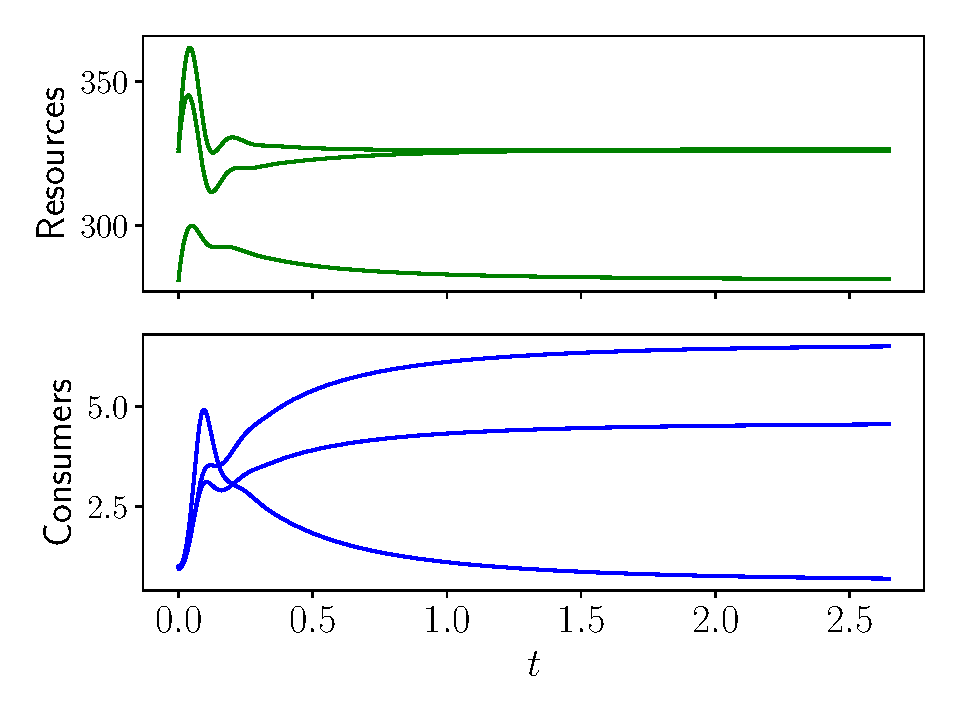
\includegraphics[width=0.6\linewidth]{Typical_time_evolution/Typical_time_evolution_resources_species_high_threshold.pdf}
% \caption{Time evolution for high coefficient threshold ($\epsilon_{\text{conv}}=10^{-1}$)}
% 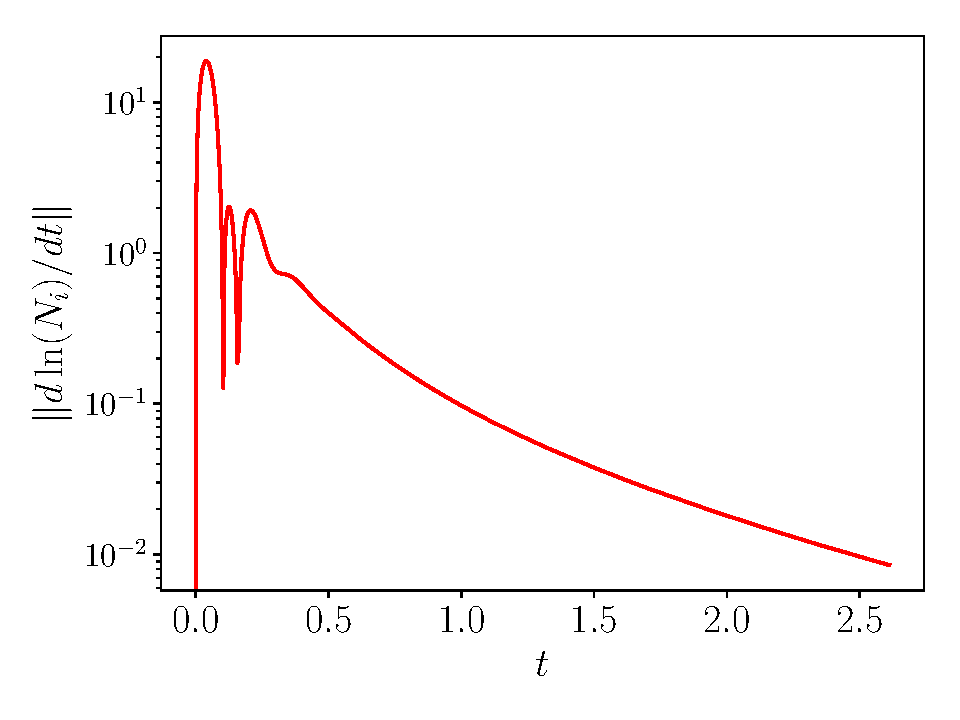
\includegraphics[width=0.6\linewidth]{figures/Typical_time_evolution/Typical_time_evolution_log_derivative_high_threshold.pdf}
% \caption{Typical convergence to judge equilibrium, we see the simulation stops at $\epsilon_{\text{conv}}=10^{-1}$}
% \end{figure}
% \begin{figure}[h!]
% \centering
% 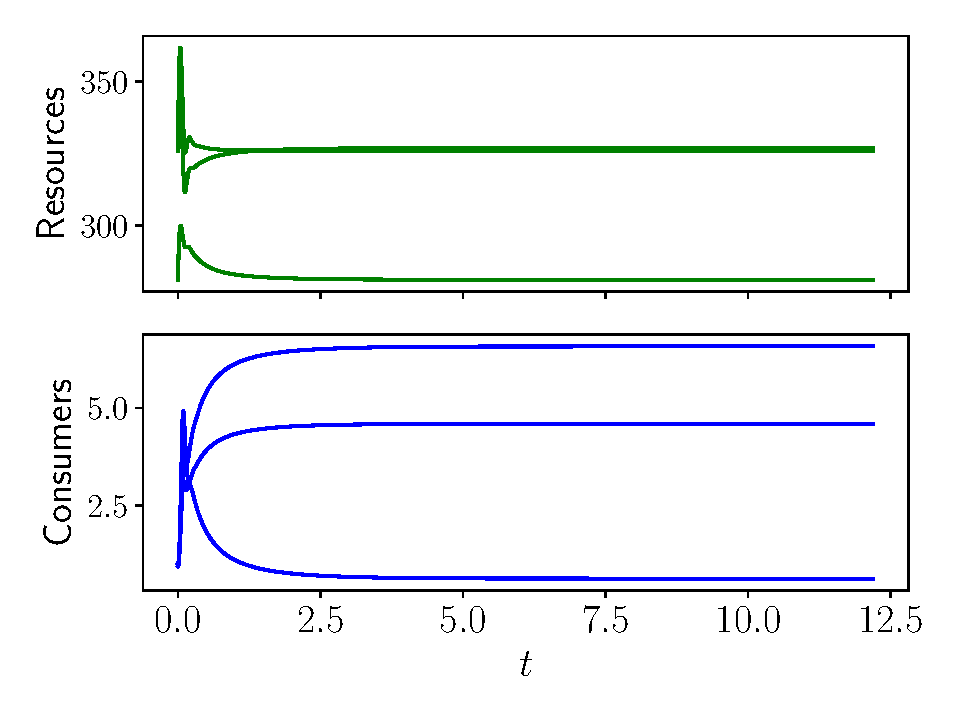
\includegraphics[width=0.6\linewidth]{Typical_time_evolution/Typical_time_evolution_resources_species_low_threshold.pdf}
% \caption{Time evolution for low coefficient threshold (more accuracy) ($\epsilon_{\text{conv}}=10^{-5}$)}
% 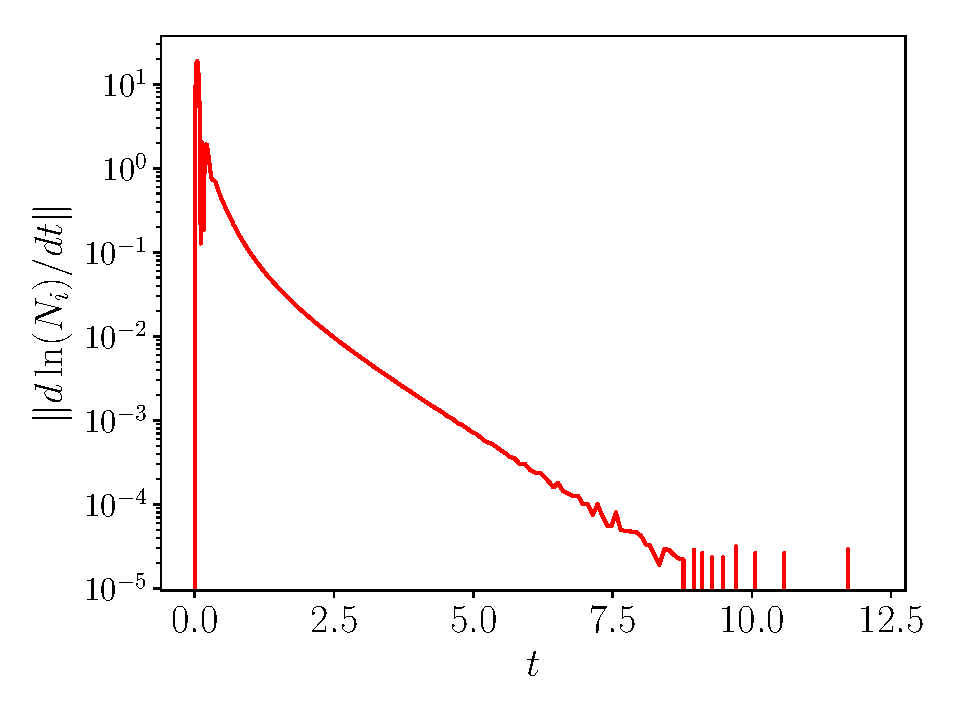
\includegraphics[width=0.6\linewidth]{figures/Typical_time_evolution/Typical_time_evolution_log_derivative_low_threshold.pdf}
% \caption{Typical convergence to judge equilibrium, we see the simulation stops at $\epsilon_{\text{conv}}=10^{-5}$}
% \end{figure}
% \subsection{Allowed parameters: syntrophy range}
% \begin{figure}[h!]
% \centering
% 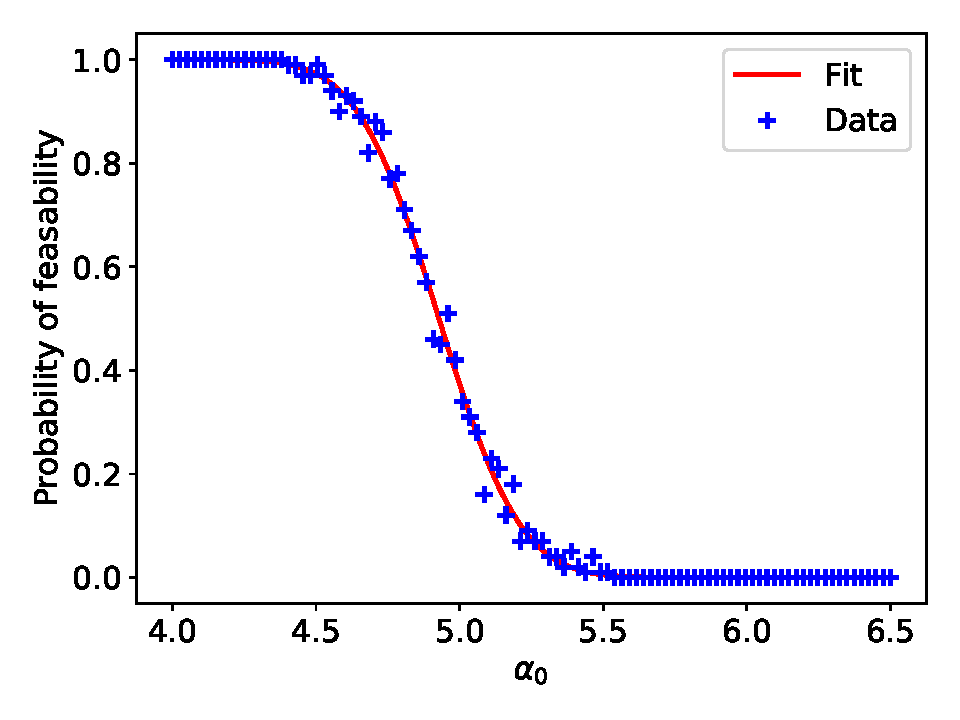
\includegraphics[scale=0.7]{figures/alpha0_probability_of_feasability}
% \caption{Typical shape of the probability of feasability for every metaparameter fixed except varying $\alpha_0$. We see that the probability of drawing a feasible system decreases sharply as $\alpha_0$ increases. A typical sigmoidal curve (here an erf function) fits the numerical data quite well.}
% \end{figure}

% \subsection{Studying the impact of the food network structure}
% \subsection{Studying the impact of syntrophy}
% We run a bunch of simulations with the following metaparameters. We made sure that these are compatible with the bounds on $\alpha_0$ Eqs.\eqref{eq: alpha bounds}.
%
% % Please add the following required packages to your document preamble:
% % \usepackage{graphicx}
% \begin{table}[h!]
% \centering
% \begin{tabular}{c|c|c|c|c|c}
% $\gamma_0$ & $\sigma_0$ & $\alpha_0$ & $R_0$ & $S_0$ & $l_0$ \\ \hline
% 1          & 1          & 0          & 300   & 1     & 11091 \\
%          & 0.75       & 0          &       &       &       \\
%          &            & 0.5        &       &       &       \\
%          & 0.5        & 0          &       &       &       \\
%          &            & 0.5        &       &       &       \\
%          &            & 1          &       &       &       \\
%          & 0.25       & 0          &       &       &       \\
%          &            & 0.5        &       &       &       \\
%          &            & 1          &       &       &       \\
%          &            & 1.5        &       &       &
% \end{tabular}
% \caption{Metaparameters used for the simulations.} \label{eq: table metaparameters used}
% \end{table}

\textbf{TO DO: write that even though feasibility does not imply dynamical stability globally does not mean that at certain points this is not true, say that large $lambda_1$ implies recovering from perturbations faster, mention somewhere that not fully feasible points not considered for dynamical stability}

We discovered in the previous section that we expect microbial communities where a large syntrophic interaction is observed to have a large consumption rate $\gamma_0$ and a small abundance of consumers at equilibrium $S_0$. It is time to work with feasible systems and investigate their dynamics. We now spend our energy on studying the local dynamical stability of feasible microbial communities. In short, we want to know what happens to them when their populations (of both resources and microbes) at equilibrium are perturbed. The question of the stability of ecosystems has always been and still remains of prime importance for ecologists and constitutes a whole scientific field. Many results have been derived, for linear systems \cite{may_will_1972}, Lotka-Volterra systems \cite{bunin_ecological_2017, takeuchi_global_1996}, mutualistic systems \cite{pascual-garcia_mutualism_2017} or MacArthur's consumer-resource model \cite{chesson_macarthurs_1990}. An important trend, which we will check with our results, is that highly connected ecological networks\footnote{This was demonstrated explicitly for mutualistic systems by \citeauthor{pascual-garcia_mutualism_2017} in \cite{pascual-garcia_mutualism_2017}.} seem to be more robust to perturbations\textbf{This was proven for structural stability, is it also true for dynamical stability?}.

In the next section we first discuss about the MCMC algorithm (Methods \ref{section: methods LRI MC solver}) designed to shape more dynamically stable systems. We then move on to study the dynamical stability of microbial communities by examining the shape of their fully dynamically stable regions, looking in what case feasibility implies dynamical stability and checking how the largest eigenvalue changes with the shape of the consumption-syntrophy network. Finally we will investigate what happens when the number of resources in the community is changed.

\subsection{LRI regime -- Outcome of the MCMC algorithm}
Methods \ref{section: methods LRI MC solver} explains how we designed an algorithm whose goal is to find, for a given consumption matrix $G$, the syntrophy matrix $A$ that should bring us closer to the satisfaction of Eq.\eqref{eq: strong LRI regime}, which we know is a dynamically stable regime. The shape of the $A$-matrix that is the outcome of the algorithm minimizes the energy $E(G,A)$ (Eq.\ref{eq: dynamical stability methods LRI MC solver energy definition}). Namely, $A$ should have the following properties:
\begin{itemize}
\item The sum of the diagonal elements of $AG$ is minimized. Because $(AG)_{\mu\mu}=\sum_{i=1}^{N_S} A_{\mu i} G_{i\mu}$ corresponds to the number of species that both consume and release resource $\mu$, we expect the algorithm to yield $A$-matrices that minimize intraspecific syntrophy.
\item The sum of the off-diagonal elements of $\abs{\alpha_0 AG-\gamma_0 R_0 G^T G}$ is minimized. This means that outside the diagonal, we should have $\frac{\alpha_0}{\gamma_0 R_0} AG \approx  G^T G$. A direct ecological interpretation is harder to draw. For a couple of different resources $(\mu,\nu)$,  $(AG)_{\mu\nu}=\sum_{i=1}^{N_S} A_{\mu i} G_{i\nu}$ is the number of species that at the same time consume resource $\nu$ and release resource $\mu$ and $(G^TG)_{\mu\nu}=\sum_{i=1}^{N_S} G_{i\mu}G_{i\nu}$ is the number of consumers that eat both $\nu$ and $\mu$. \textbf{TO DO: add something here, transition is a bit rough}
\end{itemize}
So intuitively the LRI MCMC algorithm should give us a syntrophy matrix that both limits intraspecific syntrophy and such that for every couple of different resources $(\mu, \nu)$, the number of consumers that eat both $\mu$ and $\nu$ is proportional to the number of consumers that eat $\mu$ and release $\nu$. The proportionality constant, which is the same for all $(\mu, \nu)$ is equal to the ratio of the syntrophy and consumption interactions.
 Since the connectance and the dimensions of $A$ are fixed, the number of links of $A$ is already decided and the algorithm simply determines how to optimally distribute them. Figure \ref{fig: dynamical stability results typical shape of consumption syntrophy LRI algorithm} shows that typically the algorithm will put links in a cell $(\mu,i)$ if $(i, \mu)$ is zero, meaning that not only intraspecific syntrophy tries to be avoided but also species that consume a lot of resources will tend to release few of them and vice-versa.

Figure \ref{fig: dynamical stability optimal LRI requirements met} shows that indeed we obtain for a given $G$ matrix a syntrophy matrix $A$ such that the two requirements above are best satisfied. Note that the algorithm works better for matrices with a low connectance. \textbf{TO DO: explain why}
It is worth noticing that this procedure produces highly nested syntrophy matrices (Fig.\ref{fig: dynamical stability results nestedness LRI outcome}) where only a few species produce most of the syntrophic flow. The obtained matrices have an even larger nestedness if we increase the number of resources. \textbf{TO DO : check if can speak of syntrophic overlap for nestedness of syntrophy matrix}

\subsection{Typical dynamical stability}
We observed in Results \ref{sec : feasibility without syntrophy} that, for all $(G,A) \in S_{25}$, at fixed $\alpha_0$ the metaparameters feasibility function $\mathcal{F}\left(m, G, A\right)$ has a typically sharp transition from fully feasible $(\mathcal{F}=1)$ to fully unfeasible ($\mathcal{F}=0$) regimes in the $(\gamma_0, S_0)$ plane. Figure \ref{fig : dynamical stability results typical dynamical stability function} shows that a similar although more complicated behaviour is observed in the case of the dynamical stability function $\mathcal{D}_L\left((\gamma_0, S_0, \alpha_0), G, A\right)$. On one hand, the $(\gamma_0, S_0)$ plane is split in two distinct zones, which are also separated by a very narrow boundary. The first zone is characterised by complete dynamical instability, \ie $\mathcal{D}_L =0$. On the other hand, the second zone is not described by full dynamical stability, but rather \important{almost} full dynamical stability: $\mathcal{D}_L$ is very close to but not always exactly equal to 1. The consequence is that the fully dynamically stable region $\mathcal{D}_{L,1}^{G,A}$ will be very patchy (see below for a longer discussion on this).

That patchiness could come from purely numerical effects: $\mathcal{D}_L$ is estimated by generating $N_\text{sys}$ parameters sets and counting the proportion that is dynamically stable, which inevitably leads to an uncertainty on $\mathcal{D}_L$ that could explain the patchiness. Or it could come from a genuine complicated topology of $\mathcal{D}_{L,1}^{G,A}$. In a future project, increasing $N_\text{sys}$ would allow to reduce the relative uncertainty on $\mathcal{D}_L$ and truly discover the origin of this interesting phenomenon.


\subsection{Fully dynamically stable region}\label{sec: dynamical stability methods fully dynamically stable region}
The same way we studied the fully feasible volume $\mathcal{F}_{1}^{G,A}(\alpha_0)$, we investigate now the behaviour of its special subset, the locally fully dynamically stable region $\mathcal{D}^{G,A}_{L,1}\left(\alpha_0\right)$, which is defined\footnote{A formal definition of the fully dynamically stable region $\mathcal{D}^{G,A}_{L,1}$ is provided in Methods \ref{sec: dynamical stability methods locally dynamically stable region}.} as
\begin{equation}
\mathcal{D}_{L,1}^{G,A}\left(\alpha_0\right) \defined \left\{ (\gamma_0, S_0) : (\gamma_0, S_0, \alpha_0) \in \mathcal{D}^{G,A}_{L,1} \right\}.
\end{equation}
 Intuitively, $\mathcal{D}^{G,A}_{L,1}\left(\alpha_0\right)$ corresponds to the set of all $(\gamma_0, S_0)$ such that $\mathcal{A}\left((\gamma_0, S_0, \alpha_0), G, A\right)$ is a feasible, locally dynamically stable parameters set with probability 1. Since we require $\mathcal{A}\left((\gamma_0, S_0, \alpha_0), G, A\right)$ to be feasible, it is clear that $\mathcal{D}^{G,A}_{L,1}\left(\alpha_0\right)$ is indeed a subset of $\mathcal{F}^{G,A}_1\left(\alpha_0\right)$.

 As a naive approach, one could take a look at the \important{common fully locally dynamically stable region}, which is the intersection of the $\mathcal{D}_{L,1}^{G,A}(\alpha_0) \forall (G,A) \in S_M$ (Figure \ref{fig: dynamical stability results common fully dynamically stable volume}). However, as said before, because of the patchy and heterogenous nature of each $\mathcal{D}_{L,1}^{G,A}(\alpha_0)$, we observe a very fractured and small common fully locally dynamically stable region, which is the same for all structures of $A$ considered. It has a non-zero volume for $\alpha_0=0$, but for the next point investigated $\alpha_0=\num{1.3e-3}$, no point is fully locally dynamically stable for every matrix considered, which means that the critical common syntrophy is smaller than this. This means that contrarily to the case of feasibility, we must find another, more subtle, approach to study dynamical stability. We have to consider each consumption-network individually.

As we saw, $\mathcal{D}_{L,1}^{G,A}\left(\alpha_0\right)$ is geometrically more complex than $\mathcal{F}_{1}^{G,A}\left(\alpha_0\right)$ (Figure \ref{fig: dynamical stability results local dynamical stability region for different matrices}) because of the \important{almost} fully dynamically stable points\footnote{One may argue then that we should also consider the {almost} fully dynamically stable points in the analysis. That position is intellectually appealing but would require to either work in a completely different framework or choose a ``stability threshold'' which separates almost fully feasible points from the others. The arbitrariness of said threshold (should we take into account points above $\mathcal{D}_L=0.99$? Or above $\mathcal{D}_L=0.98$? What about $0.995$?) would make such a point of view hard to hold.}.
%(which is after all not suprising, the question of dynamical feasibility is harder than the one of feasibility!)
 It may sometimes have holes, even without syntrophy, and sometimes not, even for matrices that are topologically very close. Compare for instance Fig.\ref{fig: lds region results Nest 0.35 Conn 0.2208} with Fig.\ref{fig: lds region results Nest 0.35 Conn 0.272}, these two networks have the same ecological overlap, but even though their connectance is very similar, their fully locally dynamically stable regions have a very different shape: one of them can sustain only a tiny bit of syntrophy before becoming dynamically unstable (Fig.\ref{fig: lds region results Nest 0.35 Conn 0.2208}) while the second can endure basically any feasible syntrophic interaction (Fig.\ref{fig: lds region results Nest 0.35 Conn 0.272}). As a general trend, points with a larger $\gamma_0$ and a smaller $S_0$ remain dynamically stable (Fig.\ref{fig : dynamical stability results center of stability}). The question is then: why do other points lose their dynamical stability? Is it because they become unfeasible, or do they remain feasible but become dynamically unstable?
%We required that a system had to be feasible in order to be dynamically stable, which is the mathematical equivalent of $\mathcal{D}_{L,1}^{G,A}(\alpha_0) \subset \mathcal{F}_1^{G,A}\left(\alpha_0\right)$, \ie local dynamical stability implies feasibility. We may also ask the reverse question, does feasibility imply local dynamical stability?

To answer that question, we quantify for each network $(G,A) \in S_{25}$ the \define{probability of being dynamically stable when feasible}, denoted $\text{Prob}\left(\mathcal{D}_L | \mathcal{F}\right)(G,A, \alpha_0)$. That quantity, formally defined in Appendix \ref{app : probability of being dynamically stable when feasible}, has a straight forward interpretation:
%it computes the average probability over the $(\gamma_0, S_0)$ plane that a $(\gamma_0, S_0, \alpha_0)$ point is dynamically stable if we know it is feasible. In short,
if for a certain $(G,A)$, $\text{Prob}\left(\mathcal{D}_L | \mathcal{F}\right)(G,A, \alpha_0)=x$, then a feasible $(\gamma_0, S_0, \alpha_0)$ has on average a chance $x$ to be dynamically stable\footnote{More precisely, there is a chance $x$ that a parameters set $\mathcal{A}\left((\gamma_0, S_0, \alpha_0), G, A\right)$, which we know is feasible, is also dynamically stable.}. Figure \ref{fig : dynamical stability results proba feas -> dyn sta} shows that $\text{Prob}\left(\mathcal{D}_L | \mathcal{F}\right)(G,A, \alpha_0)< 1$ $\forall (G, A) \in S_{25}$ and $\forall \alpha_0 \geq 0$. That result has a very important biological consequence : for no consumption-syntrophy network and at no syntrophy are all feasible systems dynamically stable, \ie there can always exist feasible but dynamically unstable microbial communities\footnote{This does not mean they will survive, of course, since they can vanish at any small perturbation. However it means that there is no physical law that hinders their existence: they can exist, and could appear \eg through mutation processes.}. \textbf{TO DO : if time left, do a fit of the slope but not sure if that is very relevant or what it can tell (rate at which you lose dynamical stability?)-> would show that LRI improves stuff at low connectance.}

%The answer to this is, again, unsurpisingly, ``it depends on the matrix'', as shows Figure \ref{fig: dynamical stability results local dynamical stability region for different matrices}. For instance, for $G$ with $\kappa_G=0.13$ and $\eta_G=0.1$, we have $\text{Vol}\left(\mathcal{D}_{L,1}^{G,A}(\alpha_0)\right) < \text{Vol}\left(\mathcal{F}_{L,1}^{G,A}(\alpha_0)\right) \forall \alpha_0$, which means that for this consumption matrix feasibility does not imply stability. The fully connected case gives a larger dynamically stable volume than the regime without intraspecific syntrophy which is itself better than the LRI regime. This hints that the LRI regime, despite what it was designed for, apparently does not give better results than other structures of $A$.
%On the contrary, for $G$ with $\kappa_G=0.32$ and $\eta_G=0.6$, both volumes are equal at every syntrophy that is feasible, for the three structures of $A$ considered, which shows that for this specific matrix, feasibility implies local dynamical stability.

\textbf{TO DO : talk about the fact that LRI does not improve anything}

% A good way to measure how systems react to syntrophy is to compute the \important{critical locally dynamically stable syntrophy} $\alpha_0^D(G,A)$ (see Methods \ref{sec: methods dynamical stability}). An easy way this can be done is by getting some points of the volume of $\mathcal{D}_{L,1}^{G,A}\left(\alpha_0\right)$ curve and finding its intercept to zero. Figure \ref{fig: dynamical stability results typical shrinkage of dynamical volume} shows the typical shrinkage of the fully locally dynamically stable volume.
% To find $\alpha_0^D(G,A)$ for each $G$, we fit with a linear function the last four points of the curve corresponding to Fig.\ref{fig: dynamical stability results typical shrinkage of dynamical volume} and find its intercept to zero $\alpha_0^D(G,A)$. Figure \ref{fig: dynamical stability results critical dynamical syntrophy} shows a very interesting and clear behaviour\footnote{Those results have to be taken with a grain of salt because we did not check whether $\alpha_0^D(G,A)$ was feasible, \ie the actual critical locally dynamically stable syntrophy is the minimum between the value measured in Fig.\ref{fig: dynamical stability results critical dynamical syntrophy} and the largest feasible $\alpha_0$ for that couple $(G,A)$.}: for a given connectance of the consumption matrix, systems that can sustain the largest syntrophy have a small ecological overlap. And for a given ecological overlap, systems with a larger connectance will stay stable longer under the action of syntrophy. In the end, optimal systems have a small ecological overlap and a large connectance: many resources are eaten by the consumers, but they do not share them.

Similarly to what was done for feasibility in Results \ref{sec : feasibility results influence of matrix topology}, we can measure the volume of dynamical stability \textbf{TO DO: check this is the right name} (see Appendix \ref{app: how to measure volume}) $\text{Vol}\left(\mathcal{D}_{L,1}^{G,A}(\alpha_0)\right)$ of each consumption-syntrophy network $(G,A)$. $\text{Vol}\left(\mathcal{D}_{L,1}^{G,A}(\alpha_0)\right)$ tells us what proportion of the unit square is occupied by dynamically stable $(\gamma_0, S_0)$ points and is therefore an indicator of how well communities can sustain an increase of average syntrophic strength $\alpha_0$.
Figure \ref{fig: dynamical stability results typical shrinkage of dynamical volume} shows that the dynamically stable volume typically decays in an exponential-like fashion. We inspire ourselves from the work of Results \ref{sec : feasibility results influence of matrix topology} to quantify that decay, and define the \define{dynamical stability decay rate} $d_D(G,A)$ of a consumption-syntrophy network $(G,A)$. It is obtained numerically by finding through a non-linear regression the coefficients $c_1, c_2, d_D \in \mathbb{R}^+$ that satisfy best the relation:
\begin{equation}
\text{Vol}\left(\mathcal{D}_{L,1}^{G,A}(\alpha_0)\right) \approx c_1 \exp\left(-d_D \alpha_0\right)-c_2.
\end{equation}
Much like for the corresponding discussion in the case of feasibility, $d_D(G,A)$ is an indicator of how well a consumption-syntrophy network $(G,A)$ can sustain syntrophy while remaining dynamically stable: a smaller $d_D(G,A)$ indicates a more robust network (it will take a larger syntrophy to find unstable points), a larger $d_D(G,A)$ shows the network is weak against an increase in syntrophic interaction. Figure \ref{fig: dynamical stability results dynamical decay rate FC} shows how $d_D(G,A)$ changes as a function of the characteristics of the consumption matrix $G$, $\forall G \in G_{25}$. A clear trend may be seen: in order to avoid losing dynamical stability when syntrophy is increased, a microbial community should either increase the number of average resources eaten by each consumer (\ie increase the connectance of the consumption matrix) or decrease its ecological overlap, which means that consumers should stop eating from the same resources (an intuition on why this makes sense biologically is provided in the next section \textbf{TO DO: rewrite something here better}). Figure \ref{fig : dynamical stability results decay rate away from FC case} shows how $d_D(G,A)$ changes for each matrix as different syntrophy regimes are considered. The following comments can be made\footnote{In the following, we use terms like ``is better'', ``outperforms'' or ``improves the dynamical stability'' as a way of saying ``lowers the dynamical stability decay rate compared to the FC case''.}:
\begin{itemize}
\item The NIS scenario does not significantly decrease the dynamical stability decay rate. It consistently decreases it by $\sim 5-15\%$ \textbf{TO DO: check errors}, except in the case $\kappa_G = 0.18, \eta_G=0.15$, where $d_D(G,A)$ is decreased by $\sim 30\%$.
\item The LRI scenario greatly improves ($> \sim 50\%$) the dynamical stability for consumption matrices with a very low connectance. On average, the lower the connectance, the greater the improvement. However, for larger connectances, it does not change $d_D(G,A)$ in any way.
\item The RS scenario offers the best improvement: any consumption matrix we considered got a considerably better result (at least $>\sim 20 \%$ ). At fixed connectance, the improvement is the same for every ecological overlap considered and the lower the connectance the better the improvement.
\end{itemize}
Overall, the LRI and RS scenarios offer a more significant improvement the lower the connectance of the consumption matrix. Because both have a syntrophy matrix whose connectance is equal to the one of the consumption matrix, this suggests that microbial communities which have very few syntrophic interactions (\ie $A$ has a low connectance) can remain dynamically stable with a larger average syntrophic interaction than others. Because the random structure (RS) scenario is, for a given matrix, a better improvement than LRI, we think that the syntrophy matrix should also have a lower syntrophic overlap, \ie a low nestedness\footnote{Indeed, the LRI regime has a significantly more nested syntrophy matrix compared to RS (Fig.\ref{fig: dynamical stability results nestedness LRI outcome}). At equal connectance, $A$ with the lower nestedness provides a better improvement.}.\textbf{TO DO: write why that makes sense, you depend less on the others who are changed with the perturbation}





\subsection{Largest eigenvalue of the jacobian} \label{sec: largest eigenvalue of the jacobian}
Equation \eqref{eq : dynamical stability methods fully connected metaparameters} from Methods \ref{sec : methods dynamical stability fully connected zero variance} gives a relationship that the metaparameters should approximately follow in order to give rise to locally dynamically stable systems. Although strictly speaking it is only valid for the case where both $G$ and $A$ are fully connected, we expect it to work as well when $G$ and $A$ are \important{not too far away} from the fully connected case. It tells us that in order to get more local dynamically stable systems we should\footnote{We do not focus on how $R_0$ and $l_0$ should be changed because they are always equal to $1$ for our study of feasibility and local dynamical stability. }:
\begin{itemize}
  \item Decrease $N_S$ %, $l_0$ \textbf{WEIRD RESULT: would expect that increasing l0 would make systems more dynamically stable (observed in simulations I think)}
or $\alpha_0$.
  \item If $\alpha_0 - \gamma_0 R_0 < 0$, increase $N _R$, $\sigma_0$ and $\gamma_0$.
  \item Be careful in how you handle $S_0$: %increasing $S_0$ reduces the $l_0^2/S_0$ term but increases the $N_S^2 \alpha_0^2 S_0$ term. It is very easy to show (Appendix \ref{sec: appendix how to handle S0}) that if $S_0 > l_0/(N_S \alpha_0)$ it should be decreased, and otherwise it should be increased until it reaches $l_0/(N_S \alpha_0)$.
  Appendix \ref{sec: appendix how to handle S0} shows that at very low syntrophy, we should increase $S_0$ but decrease it when $\alpha_0$ becomes very significant. Since in practice the observed feasible $\alpha_0$ are fairly low, we  should increase $S_0$ as much as possible.
\end{itemize}
Combining these considerations with the feasibility conditions Eq.\eqref{eq : fully feasible volume} we expect that -- for all other metaparameters fixed -- systems get more and more locally dynamically stable as $\gamma_0$ is increased and $S_0$ has its largest feasible value. In short, points at the upper border of $\mathcal{D}^{G,A}_{L,1}(\alpha_0)$ should have a lower and lower $\real{\lambda_1}$ as $\gamma_0$ increases. Figure \ref{fig: local dynamical stability results largest eigenvalue} shows that indeed that trend is indeed observed.
This tells us that if we keep the consumption flux $N_S \gamma_0 S_0$ constant, increasing $\gamma_0$ (and hence decreasing $S_0$) will give rise to more stable systems. Notice that contrarily to the prediction made above, increasing $\alpha_0$ does not decrease stability but increases the maximal $\abs{\real{\lambda_1}}$ observed as shows Fig.\ref{fig: dynamical stability results typical maximal eigenvalue observed varying syntrophy}. That is coupled with the already discussed shrinkage of the fully locally dynamically stable volume seen on Fig.\ref{fig: dynamical stability results shrinkage of DL1G varying syntrophy}. This means that overall increasing syntrophy makes the system \important{more stable} but at \important{fewer points}. This hints that systems in a high syntrophic regime, where consumers produce a lot of resources, should be very fine-tuned and occur for very specific consumption strength and average abundance of consumers.\textbf{TO DO : need to elaborate more?}


\subsection{The influence of the matrix dimension}
As said above, because of Eq.\eqref{eq : dynamical stability methods fully connected metaparameters}, we expect dynamical stability to improve when the number of resources is increased and the number of consumers is kept fixed. It is therefore worth briefly studying what happens when the number of resources is doubled $N_R=25 \rightarrow N_R=50$ and every other metaparameter, as well as the number of consumers, keeps the same value as before.

Figure \ref{fig: dynamical stability results typical lds region NR=50 NS=25} shows that the effect of adding resources can be quite dramatic on the stability of the system. For that specific matrix for instance, adding resources allowed for a way larger $\mathcal{D}^{G,A}_{L,1}\left(\alpha_0\right)$ at each $\alpha_0$. Interestingly, adding more resources seems to take away the patchniness of $\mathcal{D}_{L,1}^{G,A}(\alpha_0)$, which in consequence drastically changes the {common locally dynamically stable} region. Indeed $\mathcal{D}_{L,1}^{S_{50}}(\alpha_0)$ is smoother than $\mathcal{D}_{L,1}^{S_{25}}(\alpha_0)$ and can sustain a non-zero syntrophy (see the striking difference between Figure \ref{fig: dynamical stability results common fully dynamically stable volume} and Figure \ref{fig: dynamical stability results common lds volume NR=50 NS=25}). Recall that  for $N_R=25$, the critical common syntrophy was between $0$ and $\num{1.3e-3}$. It is greatly improved for $N_R=50$: between $\num{3.9e-3}$ and $\num{5.2e-3}$.

Even though more syntrophy can be sustained, it seems that the volume of $\mathcal{D}_{L,1}^{G,A}(\alpha_0)$ is smaller at $N_R=50$ than at $N_R=25$ (compare for  instance Fig.\ref{fig: dynamical stability results shrinkage of DL1G varying syntrophy NR=50} with Fig.\ref{fig: dynamical stability results shrinkage of DL1G varying syntrophy}). This is compensated by the fact that way larger eigenvalues are observed at $N_R=50$: although there are (a bit) fewer equilibrium points, these are more stable (compare Fig.\ref{fig: dynamical stability results typical maximal eigenvalue observed varying syntrophy NR=50} and Fig.\ref{fig: dynamical stability results typical maximal eigenvalue observed varying syntrophy}). This is a trend that we believe holds for all the matrices considered but a more thorough investigation should be conducted before claiming those results to be absolutely true. Since matrices are individually more locally dynamically stable,  \textbf{Is there anything more to add? I have some plots but I am not sure if they are the most relevant} \textbf{TO DO: check that last paragraph and put discussion about decay rate comparison}

\FloatBarrier
\documentclass[12pt, titlepage]{report}
\usepackage{consumer_resource_final}
\graphicspath{{./figures/}}

\begin{document}
\begin{figure}
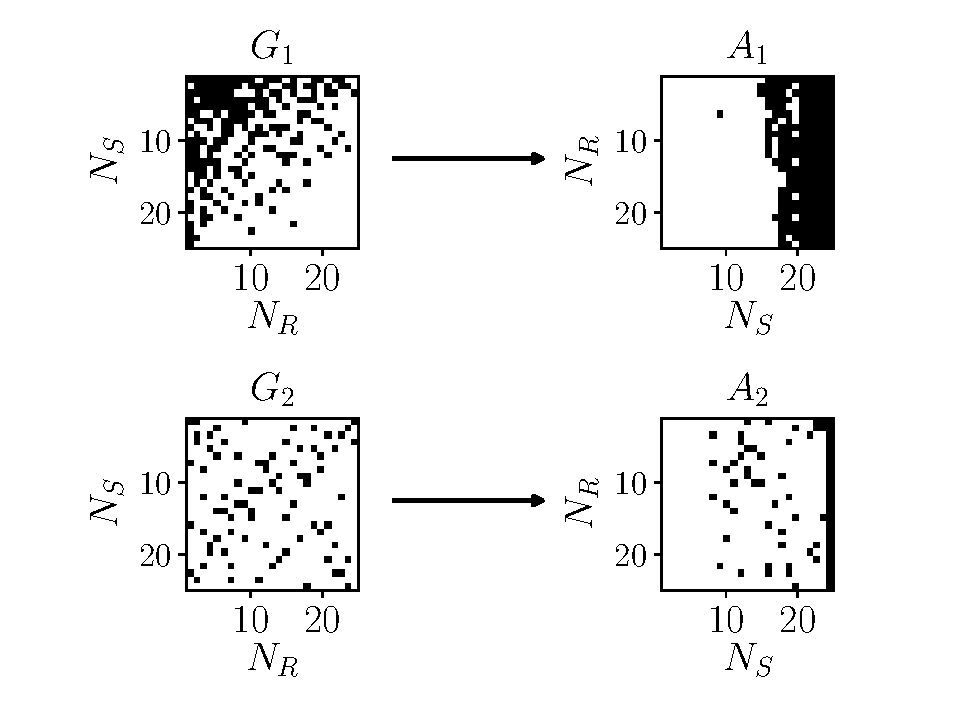
\includegraphics{typical_optimal_LRI_matrix}
\caption{Typical shape of the consumption $G_i$ and syntrophy $A_i$ matrices. The white cells symbolize a zero matrix element and the black cells, a one. $A_i$ here is the outcome of the LRI MC algorithm described in Methods \ref{section: methods LRI MC solver}. The first row has a consumption matrix with $\eta_1=0.6$ and $\kappa_1=0.32$, the LRI MC solver gives rise to a syntrophy matrix with same connectance and ecological overlap $\approx 0.85$. The second row has $G_2$ with $\eta_2=0.1$ and $\kappa_2=0.13$ and the corresponding syntrophy matrix $A_2$ has ecological overlap $\sim 0.42$. We observe that under this optimisation, species that consume few resources end up releasing many and the other way around.}\label{fig: dynamical stability results typical shape of consumption syntrophy LRI algorithm}
\end{figure}
\begin{figure}
  \begin{minipage}[c]{0.67\textwidth}
    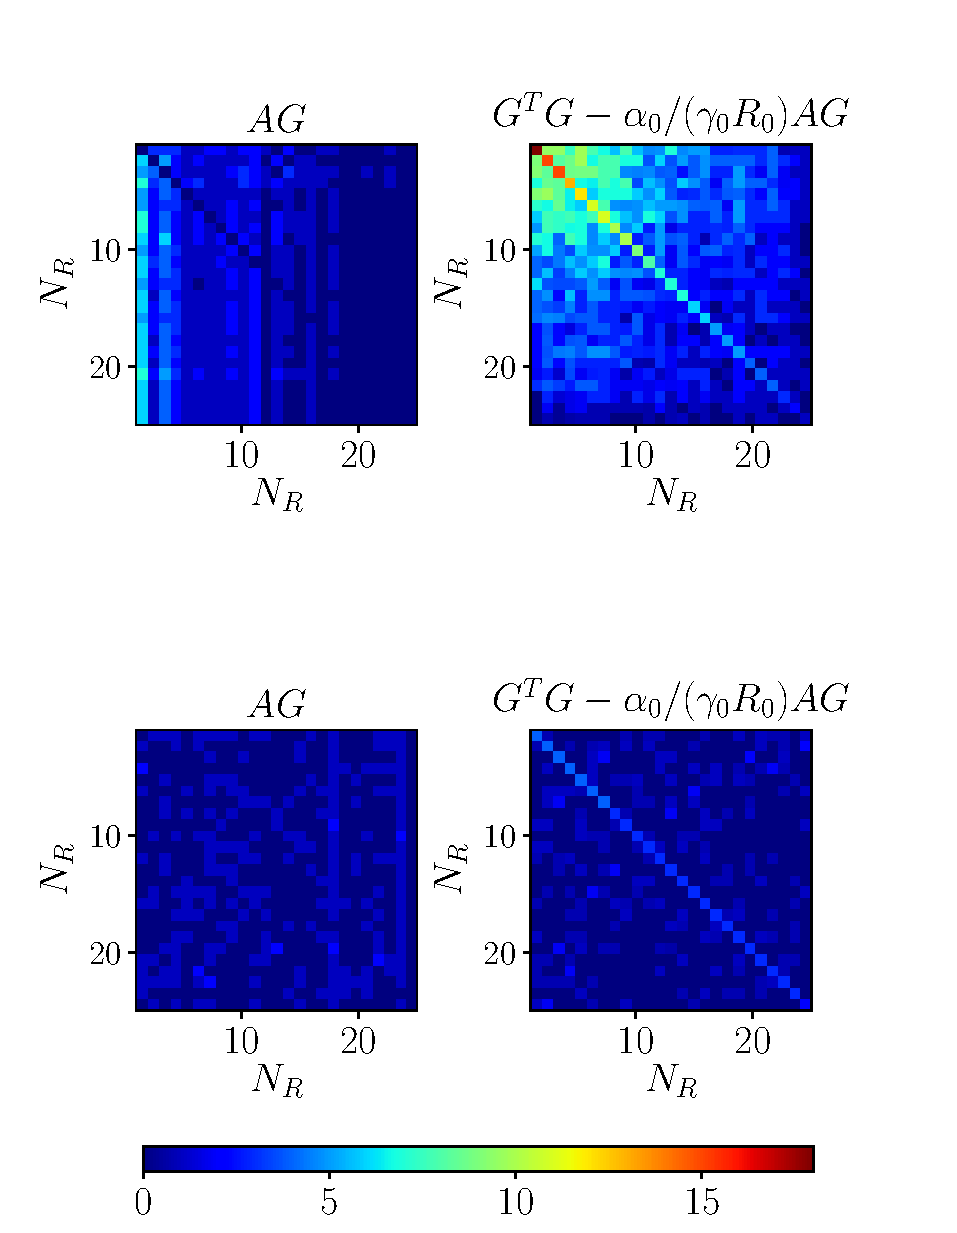
\includegraphics[width=\textwidth]{optimal_LRI_requirements}
  \end{minipage}\hfill
  \begin{minipage}[c]{0.3\textwidth}
    \caption{Plotting of $AG$ and $G^TG-\alpha_0/(\gamma_0R_0) AG$. The $A$ and $G$ matrices of the first and second rows correspond to the respective $A$ and $G$ of Figure \ref{fig: dynamical stability results typical shape of consumption syntrophy LRI algorithm}. As expected, we obtain an $A$ such that intraspecific coprophagy is limited (the diagonal of $AG$ is roughly zero) and, outside the diagonal, $G^TG-\alpha_0/(\gamma_0R_0) AG \approx 0$. Both relations are better satisfied for consumption (and hence syntrophy) matrices with a low connectance.}\label{fig: dynamical stability optimal LRI requirements met}
  \end{minipage}
\end{figure}
\begin{figure}
\captionsetup[subfigure]{captionskip = -180pt, margin = 42pt}
\hspace{-0.1\linewidth}
\subfloat[]{\includegraphics[width=0.6\linewidth]{{structure_alpha_matrix_NR25_NS25_with_nestedness}.pdf}}
\subfloat[]{\includegraphics[width=0.6\linewidth]{{structure_alpha_matrix_NR25_N25_with_connectance}.pdf}}

\hspace{-0.1\linewidth}
\subfloat[]{\includegraphics[width=0.6\linewidth]{{structure_alpha_matrix_NR50_NS25_with_nestedness}.pdf}}
\subfloat[]{\includegraphics[width=0.6\linewidth]{{structure_alpha_matrix_NR50_N25_with_connectance}.pdf}}
\caption{Properties of the syntrophy matrix against the consumption matrix. (a)-(c) Ecological overlap of $A$ as a function of the ecological overlap of $G$ for $N_S=25$ and $N_R=25$ (a) or $N_R=50$ (c). (b)-(d) Ecological overlap of $A$ as a function of the connectance of $G$ for $N_S=25$ and $N_R=25$ (b) or $N_R=50$ (d). The nestedness of the ``intraspecific syntrophy restricted'' is also plotted as a matter of comparison. As $\eta_G$ or $\kappa_G$ increase, the two results will without surprise give matrices with similar properties. \textbf{Explain this?}}
\label{fig: dynamical stability results nestedness LRI outcome}
\end{figure}
\begin{figure}
\captionsetup[subfigure]{captionskip=-225pt, margin=55pt}
\hspace{-0.1\linewidth}
\subfloat[]{\includegraphics[width=1.2\linewidth]{{probability_dynamical_stability_NR25_NS25_Nest0.5_Conn0.416_low_colorbar}.pdf}}

\vspace{-12pt}
\hspace{-0.1\linewidth}
\subfloat[]{\includegraphics[width=1.2\linewidth]{{probability_dynamical_stability_NR25_NS25_Nest0.5_Conn0.416_wo_title_high_colorbar}.pdf}}
\caption{Typical color plot local dynamical stability metaparameters function $\mathcal{D}_L$. for microbial communities with $\eta_G=0.5$ and $\kappa_G=0.42$. The color bar indicates the value of $\mathcal{D}_L\left((\gamma_0, S_0, \alpha_0), G, A\right)$ with $A$ fully connected. The plane is divided in two zones, one where $\mathcal{D}_L = 0$ and another where $\mathcal{D}_L\approx 1$ (the red and blue regions, respectively, in (a)). Upon further notice (b), it turns out the $\mathcal{D}_L \approx 1$ region is very patchy: we observe many $(\gamma_0, S_0, \alpha_0)$ configurations for which $\mathcal{D}_L$ is very close but not exactly equal to $1$. These points are \textit{almost} fully dynamically stable.} \label{fig : dynamical stability results typical dynamical stability function}
\end{figure}
\begin{figure}
\vspace{-84pt}
\hspace{-0.1\linewidth}
\includegraphics[width=1.2\linewidth]{{common_dynamical_stability_region_NR25_NS25}.pdf}
\caption{Common full local dynamical stability volume for different $A$ structures: (a) fully connected, (b) no intraspecific syntrophy and (c) LRI algorithm. The points coloured in dark red give rise to locally dynamically stable systems with probability 1 for \important{all the matrices considered}. Very few spots verify this property when there is no syntrophic interaction, and no point gives rise to a fully dynamically stable system for $\alpha_0 = \num{1.3e-3}$. This is independent of the structure of $A$ that we chose. The white points never give rise to fully dynamically stable systems.}\label{fig: dynamical stability results common fully dynamically stable volume}
\end{figure}
\begin{figure}
\captionsetup[subfigure]{captionskip = -180pt, margin = 52pt}
%\vspace{-96pt}
\hspace{-0.15\linewidth}
\subfloat[\label{fig: lds region results Nest 0.35 Conn 0.2208}]{\includegraphics[width=1.3\linewidth]{{local_dynamical_stability_wt_wc_region_NR25_NS25_Nest0.35_Conn0.2208}.pdf}}

\vspace{-44pt}
\hspace{-0.15\linewidth}
\subfloat[]{\includegraphics[width=1.3\linewidth]{{local_dynamical_stability_wt_wc_region_NR25_NS25_Nest0.35_Conn0.3216}.pdf}}

\vspace{-44pt}
\hspace{-0.15\linewidth}
\subfloat[\label{fig: lds region results Nest 0.35 Conn 0.272}]{\includegraphics[width=1.3\linewidth]{{local_dynamical_stability_wt_region_NR25_NS25_Nest0.35_Conn0.272}.pdf}}

\caption{Locally fully dynamically stable region $\mathcal{D}_{L,1}^{G,A}$ as a function of syntrophy for different matrices $G$. The white zone corresponds to points that are never fully locally dynamically stable. The colour of a given point tells until which syntrophy that point is fully locally dynamically stable, \eg
a green point is fully locally dynamically stable for $0 \leq \alpha_0 \leq \num{6.5e-3}$. Row (a) corresponds to $G$ with $\eta_G = 0.35$ and $\kappa_G = 0.23$, (b) has $\eta_G=0.35$ and $\kappa_G=0.33$ and (c) $\eta_G=0.35$ and $\kappa_G=0.27$. Even at fixed ecological overlap, different connectances of $G$ give rise to completely different systems in terms of local dynamical stability.}\label{fig: dynamical stability results local dynamical stability region for different matrices}
\end{figure}

\begin{figure}
\captionsetup[subfigure]{captionskip=-210pt, margin=28pt}
\hspace{-0.1\linewidth}
\subfloat[]{\includegraphics[width=0.6\linewidth]{{local_dynamical_stability_average_gamma0}.pdf}}
\subfloat[]{\includegraphics[width=0.6\linewidth]{{local_dynamical_stability_average_S0}.pdf}}
\caption{(a) Average consumption rate $\av{\gamma_0}_D(\alpha_0)$ and (b) average resource abundance equilibrium
$\av{S_0}_D(\alpha_0)$ as a function of syntrophy (a formal definition of $(\av{\gamma_0}_D(\alpha_0), \av{S_0}_D(\alpha_0))$ is provided in Appendix \ref{app : center of gravity local dynamical stability}). Intuitively, $(\av{\gamma_0}_D(\alpha_0), \av{S_0}_D(\alpha_0))$ represents the center $(\gamma_0,S_0)$ point of $\mathcal{D}^{G,A}_{L,1}\left(\alpha_0\right)$,  averaged over all matrices $(G,A) \in S_{25}$, or as we call it the ``\important{center of dynamical stability}''. As syntrophy increases, only points with a large consumption rate and a small resource abundance at equilibrium remain dynamically stable. The sudden drop of $\av{\gamma_0}_D$ (and rise of $\av{S_0}_D$) at $\alpha_0=\num{9.1e-3}$ is a finite-size effect. Indeed we only monitor points in the unit square $[0,1]^2$, such that the $(G,A)$ for which the center of $\mathcal{D}_{L,1}^{G,A}(\alpha_0)$ leave that zone at $\alpha_0=\num{9.1e-3}$ do not contribute to $(\av{\gamma_0}_D, \av{S_0}_D)$ anymore. Only the $(G,A)$ which previously had a lower, resp. higher, contribution to $\av{\gamma_0}_D$, resp. $\av{S_0}_D$, are taken into account, which results in that strange behaviour. The fact that $\av{\gamma_0}_D$ continues to increase (and $\av{S_0}_D$ to decrease) after that point show that this reasoning is right.}\label{fig : dynamical stability results center of stability}
\end{figure}

% \begin{figure}
% \captionsetup[subfigure]{captionskip = -230pt, margin = 50pt}
% \vspace{-96pt}
% \hspace{-0.1\linewidth}
% \subfloat[]{\includegraphics[width=1.2\linewidth]{{feasibility_vs_lds_NR25_NS25_Nest0.1_Conn0.1296}.pdf}}
%
% \hspace{-0.1\linewidth}
% \subfloat[]{\includegraphics[width=1.2\linewidth]{{feasibility_vs_lds_NR25_NS25_Nest0.6_Conn0.3168}.pdf}}
%
% \caption{Ratio of the size of the fully dynamically stable volume and the fully feasible volume for two consumption matrices $G$ (a) with $\eta_G=0.1$ and $\kappa_G=0.13$, (b) with $\eta_G=0.6$ and $\kappa_G=0.32$. We observe different behaviours for different matrices: for (a) feasibility does not imply local dynamical stability even without syntrophy (it is barely feasible but the ratio is a bit below one for $\alpha_0=0$). On the other hand, for (b) feasibility implies local dynamical stability, indeed both regions have the same volume and since $\mathcal{D}_{L,1}^{G,A}(\alpha_0) \subset \mathcal{F}^{G,A}_1(\alpha_0)$, we conclude that both are equal.}
% \end{figure}
\begin{figure}
%\captionsetup[subfigure]{captionskip=-10}
\hspace{-0.1\linewidth}
\captionsetup[subfigure]{captionskip=-140pt}
\subfloat[]{\includegraphics[width=0.4\linewidth]{{prob_dyn_stab_if_feas_NR25.0_NS25.0_Nest0.5_Conn0.416}.pdf}}
\subfloat[]{\includegraphics[width=0.4\linewidth]{{prob_dyn_stab_if_feas_NR25.0_NS25.0_Nest0.45_Conn0.384}.pdf}}
\subfloat[]{\includegraphics[width=0.4\linewidth]{{prob_dyn_stab_if_feas_NR25.0_NS25.0_Nest0.2_Conn0.0896}.pdf}}

\caption{Plot of the probability that a microbial community is dynamically stable under the assumption that it is feasible for different consumption-syntrophy networks $(G,A)$. The different lines on the same subplot show the four different $A$-scenarios. The results differ with the consumption matrix considered: (a) $\eta_G=0.5$, $\kappa_G=0.43$, (b) $\eta_G=0.45$, $\kappa_G=0.38$ and (c) $\eta_G=0.2$, $\kappa_G=0.08$. }
\label{fig : dynamical stability results proba feas -> dyn sta}
\end{figure}

\begin{figure}
\hspace{-0.1\linewidth}
\captionsetup[subfigure]{captionskip=-205pt, margin=55pt}
\subfloat[]{\includegraphics[width=0.6\linewidth]{{size_local_dynamical_stability_region_NR25_NS25_Nest0.3_Conn0.2816}.pdf}}
\subfloat[]{\includegraphics[width=0.6\linewidth]{{size_local_dynamical_stability_region_NR25_NS25_Nest0.5_Conn0.416}.pdf}}

\caption{Evolution of the dynamically stable volume $\text{Vol}\left(\mathcal{D}_{L,1}^{G,A}\left(\alpha_0\right)\right)$ (see Appendix \ref{app: how to measure volume}) with $\alpha_0$ for different $(G,A) \in S_{25}$. (a) $\eta_G=0.3$ and $\kappa_G=0.28$, (b) $\eta_G=0.5$ and $\kappa_G=0.43$. The cross-shaped points indicate the data as measured numerically while the solid lines are the corresponding exponential fit (see main text). The four colors indicate the four $A$-scenarios considered. Independent of the $(G,A)$ network, fewer points are dynamically stable as syntrophy increases.}
\label{fig: dynamical stability results typical shrinkage of dynamical volume}
\end{figure}
% \begin{figure}
% \captionsetup[subfigure]{captionskip = -185pt, margin = 52pt}
% \vspace{-84pt}
% \hspace{-0.1\linewidth}
% \subfloat[]{\includegraphics[width=0.6\linewidth]{{largest_eigenvalue_NR25_NS25_critical_alpha0_fixed_connectance_random_structure}.pdf}}
% \subfloat[]{\includegraphics[width=0.6\linewidth]{{largest_eigenvalue_NR25_NS25_critical_alpha0_fixed_nestedness_random_structure}.pdf}}
%
% \vspace{-12pt}
% \hspace{-0.1\linewidth}
% \subfloat[]{\includegraphics[width=0.6\linewidth]{{largest_eigenvalue_NR25_NS25_critical_alpha0_fixed_connectance_no_release_when_eat}.pdf}}
% \subfloat[]{\includegraphics[width=0.6\linewidth]{{largest_eigenvalue_NR25_NS25_critical_alpha0_fixed_nestedness_no_release_when_eat}.pdf}}
%
% \vspace{-12pt}
% \hspace{-0.1\linewidth}
% \subfloat[]{\includegraphics[width=0.6\linewidth]{{largest_eigenvalue_NR25_NS25_critical_alpha0_fixed_connectance_optimal_matrix}.pdf}}
% \subfloat[]{\includegraphics[width=0.6\linewidth]{{largest_eigenvalue_NR25_NS25_critical_alpha0_fixed_nestedness_optimal_matrix}.pdf}}
% \vspace{-12pt}
% \caption{Critical syntrophy $\alpha_0^D$, defined as the smallest syntrophy for which we can still find metaparameters that will give rise to fully dynamically stable systems. How $\alpha_0^D$ is estimated is explained in the main text. Errors on $\alpha_0^D$ are not plotted but are at most around $10\%$. (a)(c)(e) Evolution of $\alpha_0^D$ with ecological overlap $\eta$ at different connectance. (b)(d)(f) Evolution of $\alpha_0^D$ with connectance $\kappa$ for different ecological overlap. We observe a strong trend: for a given connectance, $\alpha_0^D$ decreases as ecological overlap increases. Also, for a given ecological overlap, $\alpha_0^D$ increases as connectance is increased.}\label{fig: dynamical stability results critical dynamical syntrophy}
% \end{figure}
\begin{figure}
\vspace{-60pt}
\hspace{-0.1\linewidth}
\captionsetup[subfigure]{captionskip=-202pt, margin=42pt}
\subfloat[]{\includegraphics[width=0.6\linewidth]{{local_dynamical_stability_NR25_NS25_dyn_stability_decay_rate_fixed_nestedness_fully_connected}.pdf}}
\subfloat[]{\includegraphics[width=0.6\linewidth]{{local_dynamical_stability_NR25_NS25_dyn_stability_decay_rate_fixed_connectance_fully_connected}.pdf}}
\caption{Dynamical stability decay rate $d_D(G,A)$ for the $A$-matrix fully connected (FC scenario) and every $G \in G_{25}$, (a) as a function of connectance $\kappa_G$ for fixed ecological overlap $\eta_G$ and (b) as a function of ecological overlap for fixed connectance. The trend confirms the previous observations: at fixed ecological overlap, a microbial community with a more connected consumption matrix will sustain a larger syntrophy (\ie have a smaller decay rate) and at fixed connectance, systems with a small ecological overlap remain dynamically stable as syntrophy grows.}\label{fig: dynamical stability results dynamical decay rate FC}
\end{figure}

\begin{figure}
\vspace{-35pt}
\captionsetup[subfigure]{captionskip = -188pt, margin = 45pt}
\hspace{-0.05\linewidth}
\subfloat[]{\includegraphics[width=0.55\linewidth]{{local_dynamical_stability_NR25_NS25_dyn_stability_decay_rate_away_from_FC_fixed_nestedness_no_release_when_eat}.pdf}}
\subfloat[]{\includegraphics[width=0.55\linewidth]{{local_dynamical_stability_NR25_NS25_dyn_stability_decay_rate_away_from_FC_syntrophy_fixed_connectance_no_release_when_eat}.pdf}}

\vspace{-12pt}
\hspace{-0.05\linewidth}
\subfloat[]{\includegraphics[width=0.55\linewidth]{{local_dynamical_stability_NR25_NS25_dyn_stability_decay_rate_away_from_FC_fixed_nestedness_optimal_matrix}.pdf}}
\subfloat[]{\includegraphics[width=0.55\linewidth]{{local_dynamical_stability_NR25_NS25_dyn_stability_decay_rate_away_from_FC_syntrophy_fixed_connectance_optimal_matrix}.pdf}}

\vspace{-12pt}
\hspace{-0.05\linewidth}
\subfloat[]{\includegraphics[width=0.55\linewidth]{{local_dynamical_stability_NR25_NS25_dyn_stability_decay_rate_away_from_FC_fixed_nestedness_random_structure}.pdf}}
\subfloat[]{\includegraphics[width=0.55\linewidth]{{local_dynamical_stability_NR25_NS25_dyn_stability_decay_rate_away_from_FC_syntrophy_fixed_connectance_random_structure}.pdf}}

\vspace{-12pt}
\caption{Relative deviation away from the $FC$ case dynamical stability decay rate as a function of the characteristics of the consumption matrix $G$. A positive $y$-coordinate means that the considered scenario provides a $d_D(G,A)$ smaller than the $FC$ case and is in consequence a sign that the network can better withstand an increase in syntrophy while remaining dynamically stable. We considered the three usual scenarios for the $A$-matrix: (a)-(b) NIS, (c)-(d) LRI and (e)-(f) RS. \textbf{TO DO: compute errors on this graph}}\label{fig : dynamical stability results decay rate away from FC case}
\end{figure}

% \begin{figure}
% \captionsetup[subfigure]{captionskip = -185pt, margin = 52pt}
% \vspace{-84pt}
% \hspace{-0.1\linewidth}
% \subfloat[]{\includegraphics[width=0.6\linewidth]{{largest_eigenvalue_NR25_NS25_critical_alpha0_fixed_connectance_random_structure}.pdf}}
% \subfloat[]{\includegraphics[width=0.6\linewidth]{{largest_eigenvalue_NR25_NS25_critical_alpha0_fixed_nestedness_random_structure}.pdf}}
%
% \vspace{-12pt}
% \hspace{-0.1\linewidth}
% \subfloat[]{\includegraphics[width=0.6\linewidth]{{largest_eigenvalue_NR25_NS25_critical_alpha0_fixed_connectance_no_release_when_eat}.pdf}}
% \subfloat[]{\includegraphics[width=0.6\linewidth]{{largest_eigenvalue_NR25_NS25_critical_alpha0_fixed_nestedness_no_release_when_eat}.pdf}}
%
% \vspace{-12pt}
% \hspace{-0.1\linewidth}
% \subfloat[]{\includegraphics[width=0.6\linewidth]{{largest_eigenvalue_NR25_NS25_critical_alpha0_fixed_connectance_optimal_matrix}.pdf}}
% \subfloat[]{\includegraphics[width=0.6\linewidth]{{largest_eigenvalue_NR25_NS25_critical_alpha0_fixed_nestedness_optimal_matrix}.pdf}}
% \vspace{-12pt}
% \caption{Critical syntrophy $\alpha_0^D$, defined as the smallest syntrophy for which we can still find metaparameters that will give rise to fully dynamically stable systems. How $\alpha_0^D$ is estimated is explained in the main text. Errors on $\alpha_0^D$ are not plotted but are at most around $10\%$. (a)(c)(e) Evolution of $\alpha_0^D$ with ecological overlap $\eta$ at different connectance. (b)(d)(f) Evolution of $\alpha_0^D$ with connectance $\kappa$ for different ecological overlap. We observe a strong trend: for a given connectance, $\alpha_0^D$ decreases as ecological overlap increases. Also, for a given ecological overlap, $\alpha_0^D$ increases as connectance is increased.}\label{fig: dynamical stability results critical dynamical syntrophy}
% \end{figure}



\begin{figure}
\vspace{-40pt}
\captionsetup[subfigure]{margin=40pt}
\hspace{-0.1\linewidth}
\subfloat[]{\includegraphics[width=1.2\linewidth]{{largest_eigenvalue_wt_NR25_NS25_Nest0.1_Conn0.1296_alpha0=0.0}.pdf}}

\vspace{-12pt}
\hspace{-0.1\linewidth}
\subfloat[]{\includegraphics[width=1.2\linewidth]{{largest_eigenvalue_wt_NR25_NS25_Nest0.1_Conn0.1296_alpha0=0.0039}.pdf}}

\vspace{-12pt}
\hspace{-0.1\linewidth}
\subfloat[]{\includegraphics[width=1.2\linewidth]{{largest_eigenvalue_wt_NR25_NS25_Nest0.1_Conn0.1296_alpha0=0.0078}.pdf}}
\caption{Largest real eigenvalue $\text{Re}(\lambda_1)$ averaged over 300 \textbf{TO DO : check number} realisations for each $(\gamma_0, S_0)$ points for the consumption matrix $G$ with consumers overlap $\eta_G = 0.1$ and connectance $\kappa_G=0.13$. The white points correspond to not fully dynamically stable systems. Each row corresponds to a different syntrophy value (a) $\alpha_0 = 0$ (no syntrophic interaction), (b) $\alpha_0 = \num{3.9e-3}$ and (c) $\alpha_0 = \num{7.8e-3}$. The different columns correspond to the different $A$ scenarios considered, which change the shape of the dynamically stable region as seen in the main text. As expected, the boundary points close to the $\gamma_0 \sim S_0^{-1}$ curve are the most stable in every situation. Points with a large $\gamma_0$ are the most stable of the unit square. }\label{fig: local dynamical stability results largest eigenvalue}
\end{figure}

\begin{figure}
\hspace{-0.1\linewidth}
\captionsetup[subfigure]{captionskip = -210pt, margin = 26pt}
\subfloat[\label{fig: dynamical stability results typical maximal eigenvalue observed varying syntrophy}]{\includegraphics[width=0.6\linewidth]{{largest_eigenvalue_varying_syntrophy_NR25_NS25_Nest0.3_Conn0.2272}.pdf}}
\subfloat[\label{fig: dynamical stability results shrinkage of DL1G varying syntrophy}]{\includegraphics[width=0.6\linewidth]{{size_local_dynamical_stability_region_NR25_NS25_Nest0.3_Conn0.2272}.pdf}}
\caption{For a consumption matrix $G$ with $\eta_G=0.3$ and $\kappa_G=0.23$. (a) Evolution of the maximal $\abs{\av{\real{\lambda_1}}}$ observed in the $(\gamma_0,S_0) \in [0,1]^2$ region. The maximal eigenvalue increases in magnitude, making the system more dynamically stable, as syntrophy increases. That trend is true for all matrices we considered. (b) Volume of $\mathcal{D}^G_{L,1}(\alpha_0)$. As syntrophy increases, fewer and fewer points become fully dynamically stable. For both figures, the different lines show the different stand for the different structure of the syntrophy matrix that we considered. \textbf{TO DO: replace this with average version}}\label{fig: results dynamical stability maximum eigenvalue observed vs size of dynamical region 25x25}
\end{figure}

\begin{figure}
\hspace{-0.15\linewidth}
\subfloat[]{\includegraphics[width=1.3\linewidth]{{local_dynamical_stability_region_NR25_NS25_Nest0.45_Conn0.3168}.pdf}}

\subfloat[]{\includegraphics[width=\linewidth]{{local_dynamical_stability_region_NR50_NS25_Nest0.45_Conn0.3328}.pdf}}
\caption{Fully dynamically stable region $\mathcal{D}^{G,A}_{L,1}$ with the three different structures of $A$ considered: fully connected (left), no intraspecific syntrophy (middle) and LRI matrix (right). The two matrices have the same ecological overlap and connectance, only the number of resources changes. (a) $G$ has $N_R=25$, $N_S=25$ and $\kappa_G=0.32$ and $\eta_G=0.45$. (b) $G$ has $N_R=50$, $N_S=25$ and $\kappa_G=0.33$ and $\eta_G=0.45$ (by lack of time, a fewer resolution on the unit square had to be taken). At $NR=50$, the fully dynamically stable region seems less fractured. The fact that more points can sustain an increased syntrophy is a trend for most of the matrices of the set. \textbf{still check this: the others are more less the same or a tad less}.} \label{fig: dynamical stability results typical lds region NR=50 NS=25}
\end{figure}
\begin{figure}
\hspace{-0.1\linewidth}
\captionsetup[subfigure]{captionskip = -210pt, margin = 26pt}
\subfloat[\label{fig: dynamical stability results typical maximal eigenvalue observed varying syntrophy NR=50}]{\includegraphics[width=0.6\linewidth]{{largest_eigenvalue_varying_syntrophy_NR50_NS25_Nest0.3_Conn0.2296}.pdf}}
\subfloat[\label{fig: dynamical stability results shrinkage of DL1G varying syntrophy NR=50}]{\includegraphics[width=0.6\linewidth]{{size_local_dynamical_stability_region_NR50_NS25_Nest0.3_Conn0.2296}.pdf}}
\caption{To be compared with Fig.\ref{fig: results dynamical stability maximum eigenvalue observed vs size of dynamical region 25x25}. The consumption matrix $G$ considered here has $\eta_G=0.3$ and $\kappa_G=0.23$. (a) Maximal average $\abs{\real{\lambda_1}}$ observed in the unit square. (b) Percentage of the unit square occupied by the fully dynamically stable region of $G$ as a function of syntrophy. The matrix considered has almost equal properties to the one in Fig.\ref{fig: results dynamical stability maximum eigenvalue observed vs size of dynamical region 25x25}, with the only difference that $N_R=50$ here. Even though the size of $\mathcal{D}_{L,1}^{G,A}$ is smaller, the eigenvalues are larger in magnitude.}
\end{figure}

% \begin{figure}
% \vspace{-72pt}
% \hspace{-0.0\linewidth}
% \subfloat[]{\includegraphics[width=\linewidth]{{largest_eigenvalue_wt_NR50_NS25_Nest0.1_Conn0.0832_alpha0=0.0}.pdf}}
%
% \vspace{-26pt}
% \hspace{-0.0\linewidth}
% \subfloat[]{\includegraphics[width=\linewidth]{{largest_eigenvalue_wt_NR50_NS25_Nest0.1_Conn0.0832_alpha0=0.0013}.pdf}}
%
% \vspace{-26pt}
% \hspace{-0.0\linewidth}
% \subfloat[]{\includegraphics[width=\linewidth]{{largest_eigenvalue_wt_NR50_NS25_Nest0.1_Conn0.0832_alpha0=0.0039}.pdf}}
% \caption{To be compared with \ref{fig: local dynamical stability results largest eigenvalue} \textbf{Is it really fair? No comparison because connectance is overall quite different and we saw that changing connectance can have quite a dramatic effect}, the zone is smaller but more stable (by a lot) can we really say this?.}\label{fig: dynamical stability results largest eigenvalue NR=50 NS=25}
% \end{figure}

\begin{figure}
\vspace{-84pt}
\hspace{-0.1\linewidth}
\subfloat[]{\includegraphics[width=0.6\linewidth]{{common_local_dynamical_stability_volume_NR50_NS25_varying_syntrophy_random_structure}.pdf}}
\subfloat[]{\includegraphics[width=0.6\linewidth]{{common_local_dynamical_stability_volume_NR50_NS25_varying_syntrophy_no_release_when_eat}.pdf}}

\centering
\subfloat[]{\includegraphics[width=0.6\linewidth]{{common_local_dynamical_stability_volume_NR50_NS25_varying_syntrophy_optimal_matrix}.pdf}}
\caption{Common fully dynamically stable volume. It is larger with a larger number of resources -> even though individually it is not always better, it is better for the worse matrices (since the common volume can handle more syntrophy)}\label{fig: dynamical stability results common lds volume NR=50 NS=25}
\end{figure}

\begin{figure}
\vspace{-84pt}
\captionsetup[subfigure]{captionskip=-202pt, margin=45pt}
\hspace{-0.1\linewidth}
\subfloat[]{\includegraphics[width=0.6\linewidth]{{local_dynamical_stability_decay_rate_50_vs_25_fixed_connectance_fully_connected}.pdf}}
\subfloat[]{\includegraphics[width=0.6\linewidth]{{local_dynamical_stability_decay_rate_50_vs_25_fixed_nestedness_fully_connected}.pdf}}

\hspace{-0.1\linewidth}
\subfloat[]{\includegraphics[width=0.6\linewidth]{{local_dynamical_stability_decay_rate_50_vs_25_fixed_connectance_no_release_when_eat}.pdf}}
\subfloat[]{\includegraphics[width=0.6\linewidth]{{local_dynamical_stability_decay_rate_50_vs_25_fixed_nestedness_no_release_when_eat}.pdf}}

\hspace{-0.1\linewidth}
\subfloat[]{\includegraphics[width=0.6\linewidth]{{local_dynamical_stability_decay_rate_50_vs_25_fixed_connectance_optimal_matrix}.pdf}}
\subfloat[]{\includegraphics[width=0.6\linewidth]{{local_dynamical_stability_decay_rate_50_vs_25_fixed_nestedness_optimal_matrix}.pdf}}

\vspace{-12pt}
\hspace{-0.1\linewidth}
% \subfloat[]{\includegraphics[width=0.6\linewidth]{{feasibility_decay_rate_50_vs_25_fixed_connectancerandom_structure}.pdf}}
% \subfloat[]{\includegraphics[width=0.6\linewidth]{{feasibility_decay_rate_50_vs_25_fixed_nestednessrandom_structure}.pdf}}

\caption{Ratio of the dynamical stability decay rates at $N_R=25$ and at $N_R=50$ as a function of the consumption matrix properties. A $y$-axis larger than $1$ means $d_D(N_R=25)$ is larger than $d_D(N_R=50)$, which means the system remains ``more'' dynamically stable as syntrophic interaction is added at $N_R=50$ compared to $N_R=25$. We considered the four usual $A$ scenarios (a)-(b) FC, (c)-(d) NIS, (e)-(f) LRI and (g)-(h) RS. On average increasing the number of resources in the system does not particularly allow microbial communities to be slightly ``more dynamically stable'' as syntrophy increases since the average ratio between the dynamical stability decay rates is very close to 1. A detailed on how the consumption matrix properties, at least connectance and ecological overlap, or the $A$-scenario precisely modify the improvement is difficult to draw from this data. \textbf{TO DO: put also the one for random structure}}
\label{fig: feasibility results feasibility decay rate NR=50 NS=25}
\end{figure}
\end{document}


\end{document}








\end{document}
